
\section{The Conversation}

\subsection{The Pitch Behind the Pitch}

They met in the quiet lounge just off the mezzanine with
velvet chairs, filtered light, and a silent espresso machine in the corner that looked sculptural but hissed like a 
snake when used. 

Hart didn’t waste time.

``I’ve seen pitch decks with less clarity than your case study,'' he said with settling into the chair opposite David 
without removing his coat.

David nodded, cautiously. The coffee in his hand was mostly cold. He wasn’t used to being approached like this.

``You built that yourself?'' Hart asked.

``Yeah,'' David said. ``Most of it.''

``What’s your background?''

``Quant. I used to build pricing models at a high-frequency shop.'' 
He hesitated. ``We blew up during the COVID carry unwind. No fraud. Just... leverage and luck.''

Hart raised an eyebrow. ``So instead of finding another job, you decided to build one.''

David half-smiled. ``Something like that.''

He explained the idea: a compliance tool --- built with the precision of trading infrastructure --- that could 
automate the data due diligence financial regulators required.  
Not just a checklist. A framework. Something that could scan model documentation, track revision histories, flag 
missing disclosures, and render it all into audit-grade reports.

Hart sat forward. His gaze sharpened.

``You’re not building regtech,'' he said. ``You’re building capacity.''

David looked puzzled.

Hart clarified: ``You’re not replacing a process. You’re replacing a personnel problem.''

He laid it out plainly. 

Most mid-tier hedge funds were boxed in. They didn’t have the budget to hire elite ML compliance engineers. 
That talent went straight to Goldman, Citadel, or was padded behind big-tech RSUs. 
The rest are hard to find, and even harder to keep.

``If you can get those shops to 80\% compliant without hiring a team to maintain the stack,'' Hart said, ``you’re not 
just solving a problem. You’re leveling the field.''

David said nothing. The hum of the nearby HVAC unit filled the pause.

Hart didn’t mind the silence. He leaned back just slightly, as if to signal: you’re the one being interviewed now.

``You won’t make them Goldman,'' he said. ``But you’ll lower the barrier to entry. That’s enough. That’s how markets shift.''

Then, softer, more pointed:

``You don’t need my validation. You’ve got product. What you need is volume.''

He tapped the card he’d laid on the table.

``I know who needs this. Let’s talk.''

\medskip

\begin{HistoricalSidebar}{The Anatomy of a Value Proposition: Why Some Products Land and Others Stall}

  A \textbf{value proposition} is not what a product \textit{does}. It's what it \textbf{solves}. And in markets 
  crowded with technical talent and noise, clarity about that distinction can determine whether a startup takes 
  off or disappears.
  
  \medskip
  
  In startup mythology, product-market fit often gets all the attention. But what gets overlooked is \textbf{problem-founder fit}: 
  whether the founder truly understands the pain they’re solving — and who has it.
  
  \medskip
  
  \textbf{Successful Example: Stripe (2010)}  
  Most payment platforms in 2010 focused on buyers. Stripe targeted \textit{developers} — the engineers tasked with integrating 
  payment APIs. Their value proposition wasn’t “payments made easy,” it was:  
  \textit{“You can deploy a full payments stack in 7 lines of code.”}  
  The problem wasn’t payments — it was \textbf{friction}. Stripe solved for the person who had to ship working code by the end 
  of the week.
  
  \medskip
  
  \textbf{Failed Example: Color Labs (2011)}  
  Color Labs raised \$41 million to launch a social photo app that let users share images with people nearby. The technology 
  was novel — using GPS and proximity to build social networks on the fly — but the value proposition was fuzzy:  
  \textit{“Take pictures together in real-time.”}  
  What problem did it solve? Who needed it? Why now? Users didn’t know. Neither did investors by the time it folded.
  
  \medskip
  
  \textbf{Gray Zone Example: Juicero (2013)}  
  Juicero’s product — a \$400 cold-press juicer — was marketed as a health-tech device with subscription-based juice packets. 
  On paper, it sounded modern and slick. But once people realized you could squeeze the packets by hand, the core value 
  proposition evaporated:  
  \textit{It wasn't about juice. It was about perceived luxury.}  
  The mismatch between actual utility and projected status killed the brand.
  
  \medskip
  
  \textbf{The lesson?}  
  Value proposition design isn’t about feature lists — it’s about mapping your product to a very specific bottleneck in someone 
  else’s world. The sharper the bottleneck, the clearer the value.
  
  \medskip
  
  That’s why Hart zeroed in on David’s tool. Not because it was novel, but because it solved a specific institutional constraint:  
  “Get to 80\% compliance without hiring.”
  
\end{HistoricalSidebar}

\subsection{Flattening the Curve}


The second pour of scotch had softened the edges.

They were seated in the lounge of the downtown private club with it's brushed brass and low lighting. It was the kind 
of place designed to look expensive without feeling new. Outside, the city buzzed with Thursday night urgency, but inside, 
everything moved slower. Intentional. The table was marble, veined with gold, chilled to the touch. The waiter had 
long since faded into the background.

The pitch was over. Now came the calculus.

Hart leaned in, elbows on the stone.

``You’re not building a compliance product,'' he said. ``You’re building a keycard.''

David blinked once, slowly. ``Keycard?''

Hart didn’t smile. He clarified without condescension:

``You’re not solving for oversight. You’re solving for access. You’re handing mid-tier funds a way into a market they were 
never allowed to touch.''

On the other side of the table, Penn looked up from the term sheet he’d been annotating with a silver Montblanc. He didn’t 
interrupt. Just listened.

Hart continued:

``High-frequency trading isn’t locked off because of regulation. It’s locked off because of stack complexity. 
Infrastructure. Latency. State handling. Data streaming. And yeah, regulatory overlays, but those come after.''

David nodded slowly, his fingers wrapped around the base of his glass. ``Most of them don’t even try. The bar’s too high.''

``Exactly,'' Hart said. ``They’re priced out by the engineering curve. Not the compliance curve. You flatten that curve, you 
open the gate.''

The ice in David’s glass cracked gently, like it had been waiting for the moment.


\medskip

\begin{TechnicalSidebar}{Barriers to Entry and Why Most Funds Stay Out}

  A \textbf{barrier to entry} is anything that prevents a new player from entering a market and competing effectively.  
  These barriers aren’t always regulatory. In fintech and high-frequency trading (HFT), they’re often 
  \textit{technical, infrastructural, or cultural}.
  
  \medskip
  
  \textbf{In HFT and ML-driven trading, the primary barriers include:}

  \medskip
  
  \begin{itemize}
    \item \textbf{Stack Complexity:}  
    Millisecond-level latency requirements, real-time introspection, and fault-tolerant event handling pipelines.
  
    \item \textbf{Talent Scarcity:}  
    Engineers who understand trading systems, compliance hooks, and low-level performance tuning are rare — and expensive.
  
    \item \textbf{Regulatory Overlay:}  
    Once infrastructure exists, it must also meet legal standards — audit logs, fair execution, capital disclosures — without slowing performance.
  
    \item \textbf{Reputational Signaling:}  
    Even with a working stack, institutional allocators are wary of unknown platforms without validation from top-tier logos.
  \end{itemize}
  
  \medskip
  
  \textbf{The Result?}  
  Even well-capitalized funds avoid building from scratch.  
  Not because they don’t want to — but because the path to parity is too steep, too slow, and too expensive.
  
  \medskip
  
  \textbf{The strategic unlock?}  
  Build a system that \textit{collapses the engineering barrier} without compromising regulatory posture.  
  Suddenly, you’re not selling software. You’re selling \textbf{access}.
  
\end{TechnicalSidebar}


\medskip

The scotch had mellowed, but the air stayed sharp from the clarity that only comes when no one’s 
pretending anymore. The room had the lacquered hush of old money: recessed lights, no music, and walls lined with abstract 
art chosen more for tax deduction than taste.

Outside, the city blurred under halogen and mist, but in here, everything had slowed to a crisp, analytical tempo.

David described the pipeline again as a vertical-integration play:  
an internal model engine, backtesting under stress scenarios, pipeline introspection, and compliance hooks all rendered 
into modular, containerized deploys.

``You don’t build a product,'' Hart said. ``You build entry velocity.''

David raised an eyebrow. ``Meaning?''

Hart smiled faintly, resting his glass on the marble.

``Meaning they can go from zero to trading without hiring Citadel’s shadow stack.''

Penn folded the term sheet and tapped the cover with two fingers, like sealing an envelope.

``So you’re not selling features. You’re selling qualification.''

``Exactly,'' Hart replied. ``Most people fail the entry exam. You let them cheat.''

Hart pivoted, now sketching the business model in the air with his hand.

``You don’t price it like a SaaS tool. You price it like a futures contract.  
You’re not charging for usage. You’re charging for entry rights.''

David stayed silent. This wasn’t how he had framed it, but it clicked.  
Not a toolkit. Not a reg layer.

A gateway.

And gateways? Those get priced by what they unlock.



\subsection{Napkin Math and Synthetic Margins}

The bar was dim, upscale but unpretentious. It was the kind of place where the lighting was low enough to suggest intimacy, 
but not so low that you couldn’t read a term sheet. A jazz trio murmured in the corner, and the leather booths smelled 
faintly of cedar and citrus polish.

Hart pulled a cocktail napkin toward him and clicked a pen from his jacket. He didn’t bother asking for a fresh sheet of paper.

``Let’s run the numbers,'' he said, scribbling a row of assumptions down the margin. ``Not investor math. 
Fermi math.''

Morales grinned and leaned in. ``Back-of-the-envelope?''

``Always,'' Hart said. ``It’s not about precision. It’s about order of magnitude sanity.''

He drew three columns: headcount, compliance burden, deployment velocity.

``Say a fund with \$300 million AUM wants to scale into synthetic credit. Normally they’d need --- what? --- five 
headcount just to maintain reporting compliance?''

\medskip

\begin{TechnicalSidebar}{What is Synthetic Credit?}

  \textbf{Synthetic credit} refers to exposure to credit risk through financial derivatives—rather than through direct 
  ownership of bonds or loans.

  \medskip
  
  Unlike traditional credit instruments (e.g., corporate bonds), synthetic credit positions are created using tools 
  such as:

  \medskip
  
  \begin{itemize}
    \item \textbf{Credit Default Swaps (CDS):}  
    A CDS functions like credit insurance. The buyer pays a regular premium to the seller, and in return, gets 
    compensated if a third-party borrower (like a company or government) defaults.  

    \medskip
  
    \textit{Example:} It's like paying monthly insurance on a neighbor’s mortgage. However, you don’t own the house, but 
    you’ll get a payout if they default on the loan.


    \medskip
  
    \item \textbf{Total Return Swaps (TRS):}  
    In a TRS, one party agrees to hand over the total return (interest + price appreciation) from a credit asset 
    in exchange for a fixed or floating payment.  

    \medskip
  

    \textit{Example:} Imagine you own a risky bond, but instead of collecting its unpredictable income, you trade 
    it for steady monthly rent and give someone else the upside (and risk) in exchange for certainty.


    \medskip
  
    \item \textbf{Structured Notes or Options:}  
    These are custom-built financial products based on baskets of credit indices or portfolios, often with embedded 
    features like leverage or downside protection.  

    \medskip
  

    \textit{Example:} Think of it like a chef's tasting menu. You're not just betting on one credit, but on a handpicked 
    combo of bonds or indices, with special ingredients like caps, floors, or trigger conditions that shape how 
    (and if) you get paid.
  \end{itemize}

  \medskip
  
  These instruments allow funds to scale exposure rapidly without purchasing underlying assets. They're cheaper, faster, 
  and more capital-efficient, but also more opaque.

  \medskip

  \begin{figure}[H]
    \centering
    \resizebox{0.92\textwidth}{!}{%
      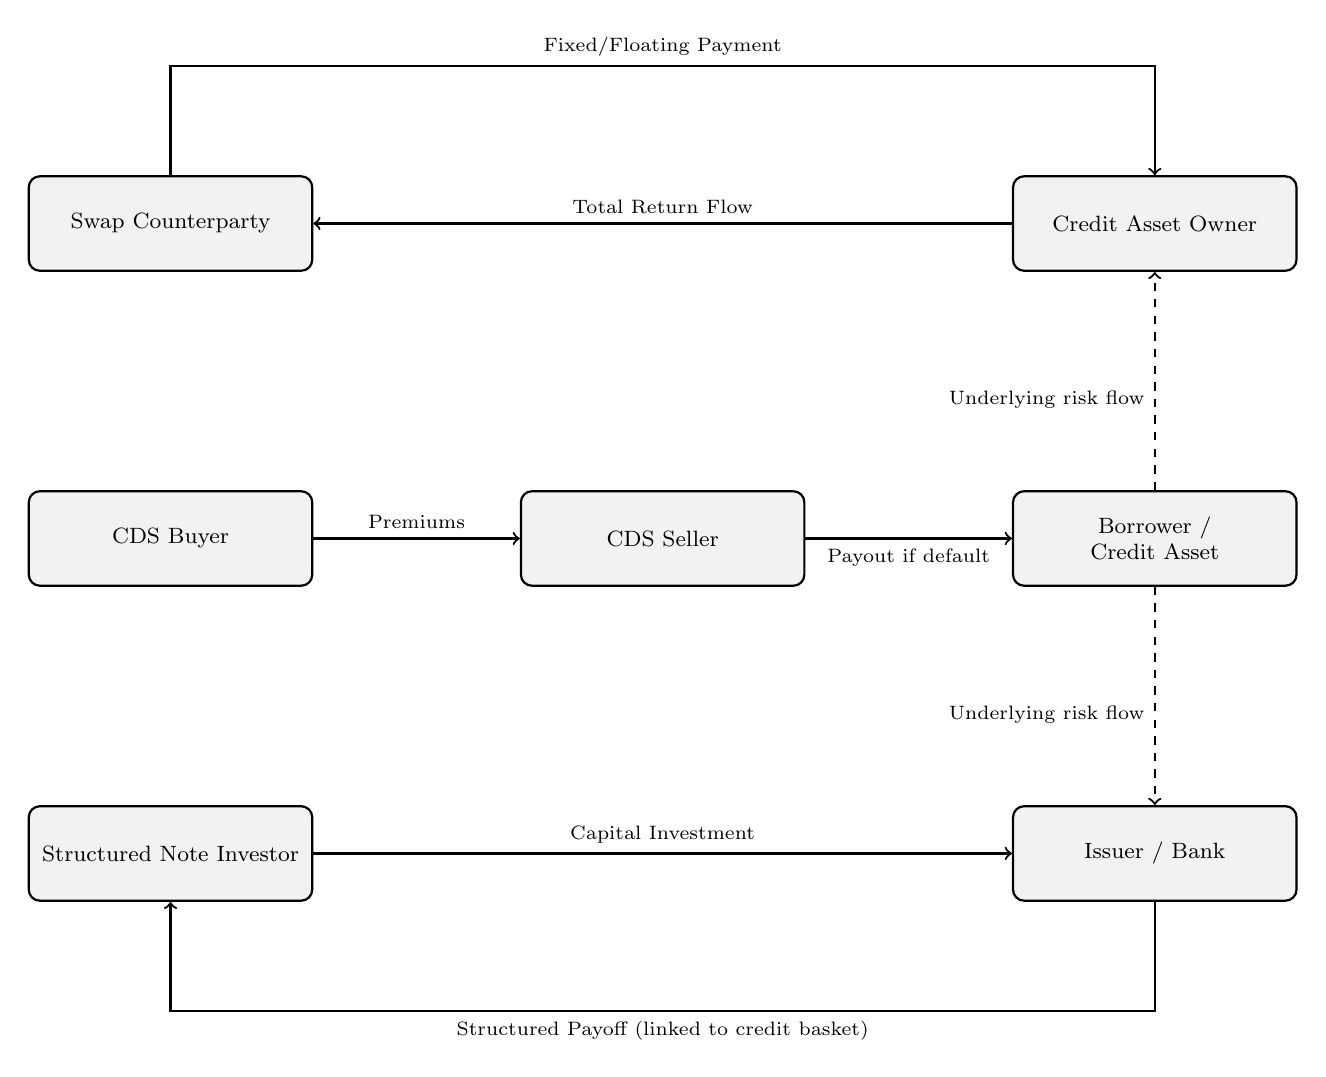
\begin{tikzpicture}[
        font=\footnotesize,
        box/.style={draw, thick, rounded corners, minimum width=3.6cm, minimum height=1.2cm, align=center, fill=gray!10},
        arrow/.style={->, thick},
        note/.style={font=\scriptsize\itshape},
        x=2.5cm, y=2cm
      ]
  
      % Source of risk
      \node[box] (borrower) at (5,0) {Borrower /\\Credit Asset};
  
      % CDS
      \node[box] (cdsbuyer) at (0,0) {CDS Buyer};
      \node[box] (cdsseller) at (2.5,0) {CDS Seller};
  
      \draw[arrow] (cdsbuyer) -- node[above] {\scriptsize Premiums} (cdsseller);
      \draw[arrow] (cdsseller) -- node[below] {\scriptsize Payout if default} (borrower);
  
  
      % TRS
      \node[box] (trsasset) at (5,2) {Credit Asset Owner};
      \node[box] (trsparty) at (0,2) {Swap Counterparty};
  
      \draw[arrow] (trsasset) -- node[above] {\scriptsize Total Return Flow} (trsparty);
      \draw[arrow] (trsparty) 
        -- ++(0, 1) coordinate (drop)
        -- ++(+2.5, 0) coordinate (midpoint)
        -|
        (trsasset);

      \node[above] at (midpoint) {\scriptsize Fixed/Floating Payment} (trsasset);
  
  
      % Structured Notes
      \node[box] (investor) at (0,-2) {Structured Note Investor};
      \node[box] (issuer) at (5,-2) {Issuer / Bank};
  
      \draw[arrow] (investor) -- node[above] {\scriptsize Capital Investment} (issuer);
      \draw[arrow] (issuer) 
        -- ++(0, -1) coordinate (drop)
        -- ++(-2.5, 0) coordinate (midpoint)
        -|
        (investor);
      \node[below] at (midpoint) {\scriptsize Structured Payoff (linked to credit basket)};


  
  
      % Borrower arrow
      \draw[arrow, dashed] (borrower) -- node[below left] {\scriptsize Underlying risk flow} (trsasset);
      \draw[arrow, dashed] (borrower) -- node[below left] {\scriptsize Underlying risk flow} (issuer);

      %\node[note] at (-2,2.6) {CDS shifts default risk};
      %\node[note] at (4,0.8) {TRS swaps performance for certainty};
      %\node[note] at (2.5,-3.3) {Notes repackage risk into custom products};
  
      \end{tikzpicture}%
    }
    \caption{How Credit Derivatives Distribute or Transform Credit Risk}
  \end{figure}

  \medskip
  
  \textbf{Why use it?}  

  \medskip

  Funds deploy synthetic credit to:

  \medskip
  
  \begin{itemize}
    \item Express directional credit views without taking balance sheet risk
    \item Hedge credit portfolios with speed and precision
    \item Amplify leverage in a regulatory-compliant wrapper
  \end{itemize}

  \medskip
  
  \textbf{The tradeoff:}  
  
  \medskip

  While synthetic credit boosts flexibility and velocity, it can distort actual exposure metrics. During stress events, 
  the correlation between synthetic and physical markets can break down—causing ``drift'' between expected protection 
  and realized loss.

  \medskip
  
  This divergence played a central role in multiple financial dislocations, including the 2008 collapse of AIG’s CDS 
  book, and more recently, in smaller liquidity ruptures triggered by undercapitalized synthetic tranches.
  
\end{TechnicalSidebar}

\medskip

``Minimum,'' David said. ``Assuming no turnover.''

``Right,'' Hart said, underlining the number. ``Now suppose your pipeline replaces three of those roles 
and reduces latency by 60\%. What does that buy them?''

``Speed to market. And internal optics.''

Hart nodded. ``And optics translate into allocation. Faster compliance means faster scaling.''

He tapped the napkin, now smudged with numbers and ink streaks.

``That’s your margin,'' he said. ``Not in features. In time arbitrage.''

David stared at the scribbled napkin. The math was loose. But the logic was airtight.

He didn’t need a calculator. He needed a clock.

And Hart had just reset it.

\medskip


\begin{HistoricalSidebar}{Fermi Estimation: How Atomic Physics Became a Quant Interview Question}

  In July 1945, at the Trinity nuclear test site in New Mexico, Enrico Fermi stood among a group of physicists waiting for 
  history to unfold.  
  As the countdown to the first atomic explosion reached zero, Fermi performed an odd, almost casual act: he dropped small 
  scraps of paper.
  
  \medskip
  
  When the shockwave from the detonation reached him, he observed how far the papers had traveled.  
  From that simple displacement, he estimated the blast yield at approximately 10 kilotons of TNT.
  
  \medskip
  
  Official measurements later put it at about 18.6 kilotons — meaning Fermi, with no instruments and only a handful of confetti, 
  was within a factor of 2.
  
  \medskip
  
  This moment became legend: not because of the accuracy, but because of the method.  
  Fermi didn’t measure. He decomposed the problem into approximate parts — what we now call a \textbf{Fermi estimate}.
  
  \medskip
  
  \textbf{Fermi estimation} is a mental technique for approximating a quantity using only logical reasoning and 
  order-of-magnitude assumptions.  
  It’s the art of going from ``I have no idea'' to ``I have a rough sense'' using structured guesswork.
  
  \medskip
  
  \textbf{The canonical example:}  
  How many piano tuners are there in Chicago?

  \medskip
  
  \begin{itemize}
    \item Population of Chicago: \textasciitilde3 million  
    \item Average household size: 2.5 $\Rightarrow$ 1.2 million households  
    \item Households with pianos: \textasciitilde1 in 20 $\Rightarrow$ 60,000 pianos  
    \item Tunings per piano per year: 1  
    \item Total tunings: 60,000/year  
    \item A tuner can do 4 jobs/day, 5 days/week, 50 weeks/year = 1,000 tunings/year  
    \item Needed tuners: 60,000 / 1,000 = \textbf{60 piano tuners}
  \end{itemize}
  
  \medskip
  
  Of course, the real number might be 50 or 80. But that’s not the point.  
  What matters is the \textbf{reasoning}.
  
  \medskip
  
  That’s why Fermi questions became a staple of quant interviews, startup pitches, and market strategy sessions.  
  They don’t test precision.  
  They test \textbf{decomposition, intuition, and the courage to guess}.
  
  \begin{quote}
  \textit{“All models are wrong,”} the saying goes, \textit{“but some are useful.”}  
  Fermi estimates live in that exact margin.
  \end{quote}
  
  \medskip
  
  Whether estimating nuclear yields or billion-dollar TAMs, Fermi logic reminds us:  
  You don’t need perfect data to make a high-quality decision.  
  You just need the guts to bound the problem — and the clarity to own your assumptions.
  
\end{HistoricalSidebar}
  

\subsection{A Market Just Deep Enough}

The napkin was already cluttered, but Hart kept writing.

``There are about 5{,}000 hedge funds globally,'' he said, thinking aloud. ``Call it 2{,}000 
that are small-to-mid tier. The kind that can’t build their own infra stack.''

David leaned over the table.

``Assume 5\% are actively trying to expand into ML-based quant. That’s 100 funds.  
We could reasonably sell to half over five years if we build a reputation. So 50 logos?''

Hart nodded.

``Call it 10 the first year. If they pay \$250{,}000 each, that’s \$2.5 million topline.  
Think pilot licenses, integration, and support.''

David sipped his drink. ``And that’s before we license the IP or run API-based usage tiers.''

``Exactly,'' Hart said. ``If even 20\% of the target market scales usage and upgrades to \$500{,}000 per year,  
we’re looking at \$10–15 million annual run rate within 3 years.''

David tapped the napkin.

``So you frame it like this:''

The napkin was a mess — arrows, margins crowded with dollar signs, numbers scribbled into a funnel. But as David 
stared at it, something clicked.

It reminded him of how he got his first job.

Not from a polished resume — but from answering a market sizing question scrawled on the back of a flyer at a campus event.
“Size the market for enterprise AI in logistics.” No internet. No prep.

He broke it down on the spot — industry size, adoption curve, price points — drew a funnel, gave a number.
Rough. Fast. Believable.

That got him in the door.

Now here he was, years later, doing the same thing:
\begin{itemize}
    \item 2,000 funds 
    \item 5\% early adopters 
    \item 50 clients 
    \item \$250k each.
\end{itemize}

No slides. Just ink and instinct.

And for a moment, he smiled.
The math hadn’t changed.
Only the stakes had.

\medskip

\begin{figure}[H]
    \centering
    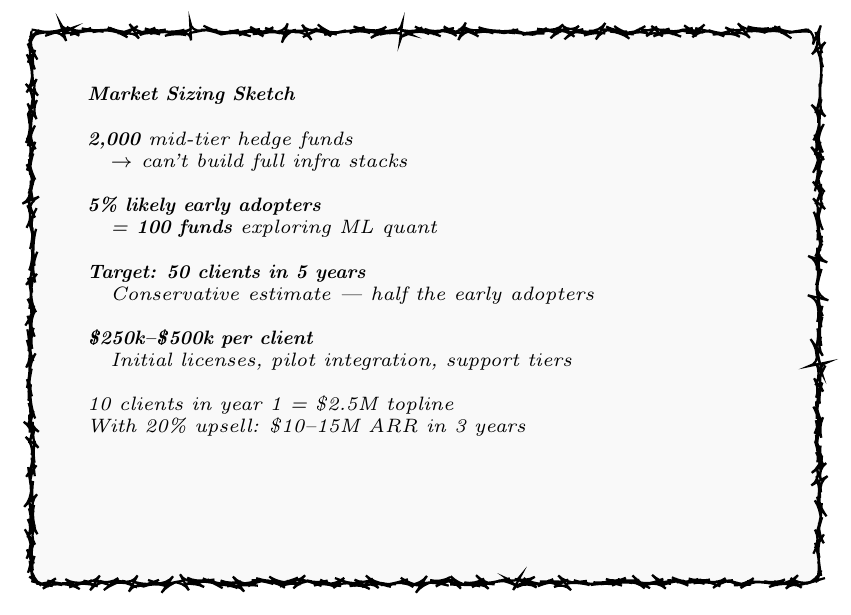
\begin{tikzpicture}[
      font=\footnotesize,
      fuzz/.style={draw=black, thick, rounded corners, fill=gray!5, decorate, decoration={random steps, segment length=2pt, amplitude=1pt}},
      txt/.style={align=left, font=\scriptsize\itshape},
    ]
  
    % Napkin box
    \node[fuzz, minimum width=10cm, minimum height=7cm, anchor=north west] (napkin) at (0,0) {};
  
    % Content inside
    \node[txt, anchor=north west] at ([xshift=0.6cm, yshift=-0.6cm]napkin.north west) {
      \textbf{Market Sizing Sketch} \\
      \\
      \textbf{2{,}000} mid-tier hedge funds \\
      \quad $\rightarrow$ can't build full infra stacks \\
      \\
      \textbf{5\% likely early adopters} \\
      \quad = \textbf{100 funds} exploring ML quant \\
      \\
      \textbf{Target: 50 clients in 5 years} \\
      \quad Conservative estimate — half the early adopters \\
      \\
      \textbf{\$250k–\$500k per client} \\
      \quad Initial licenses, pilot integration, support tiers \\
      \\
      \textit{10 clients in year 1 = \$2.5M topline} \\
      \textit{With 20\% upsell: \$10–15M ARR in 3 years}
    };
  
    \end{tikzpicture}
    \caption{Napkin Summary: Market sizing and revenue projection for ML quant infrastructure sales.}
\end{figure}

\medskip

Hart leaned back, smiling.

``Exactly. Market isn’t huge. But it’s deep. It's high trust, high margin, and high retention.  
And once the first five logos land, the rest follow.  
Because nobody wants to be the last quant fund without a real-time audit layer.''

David nodded slowly.

``And if you wrap the IP into a licensing structure, the revenue multiple goes from 5x to 12x overnight.  
TAM is maybe \$500 million globally. We don’t need it all. We just need the perception that we could take 10\%.''

Hart smirked.

``And that’s how you Fermi your way into a \$50 million valuation in the first year after deployment.''


\medskip

\begin{TechnicalSidebar}{Business Viability, Payback Period, and Why VCs Care About Speed}

  One of the most underrated metrics in early-stage venture capital isn’t TAM, burn rate, or even ARR.  
  It’s \textbf{payback period} — the time it takes for a new customer to generate enough revenue to cover their own acquisition cost.
  
  \medskip
  
  \textbf{Payback Period Formula:}
  \[
  \text{Payback Period} = \frac{\text{Customer Acquisition Cost (CAC)}}{\text{Gross Margin from Customer per Month}}
  \]
  
  \medskip
  
  If it costs \$50,000 to close a deal and that customer brings in \$25,000 per month in margin,  
  the payback period is 2 months.
  
  \medskip
  
  \textbf{Why it matters:}
  
  \begin{itemize}
    \item Short payback = fast reinvestment cycles. A startup can recycle revenue into more growth without needing new funding.
    \item Long payback = higher risk. The startup must float costs for months (or years) before breakeven.
    \item For VC firms, short payback implies \textbf{capital efficiency} — every dollar deployed drives quicker returns.
  \end{itemize}
  
  \medskip
  
  In the case of Hart and Morales’ strategy:

  \medskip
  
  \begin{itemize}
    \item Each client pays \$250K to \$500K annually.
    \item The product is deployed quickly — modular, containerized, low-integration overhead.
    \item Gross margins exceed 80\%, given the IP-heavy, low-support model.
  \end{itemize}
  
  \medskip
  
  Even assuming \$50K to acquire each customer, they break even within 3 months.  
  That puts them in elite territory — where CAC is recouped before the second quarter, and LTV/CAC ratios can exceed 8x.
  
  \medskip
  
  \textbf{The VC view:}  
  This isn’t just a niche tool. It’s a high-trust, high-ticket product with low churn and fast returns.
  
  \begin{quote}
  \textit{In venture math, velocity beats volume.  
  A product that pays itself back in 90 days can be scaled   
  (even before it's perfect).}
  \end{quote}
  
\end{TechnicalSidebar}
  

\medskip

\subsection{Narrative as a Moat}


Hart was drawing boxes on the napkin again.

``Let’s scale this. Think beyond hedge funds. Who else needs this?''

David didn’t hesitate.  
``Anyone algorithmically allocating capital under regulatory pressure:
  Banks with quant desks;  
  Sovereign wealth arms; 
  Insurance and pensions migrating into automated trading; 
  Even crypto funds trying to look institution-grade''

Hart tapped his pen twice. ``So what’s the real market size?''

David ran the numbers aloud.

``Globally? Maybe 30{,}000 institutional allocators.  
Say 10{,}000 are actively integrating ML or automation over the next five years.  
Conservatively, 20\% are in position to buy infra — that’s 2{,}000 serious prospects.''

Hart grinned. ``Then we blitz it.''

David raised an eyebrow. ``You’re saying go wide before we even optimize?''

``Exactly,'' Hart replied. ``Control’s a second-mover problem.  
Right now, we’re building surface area. \$500K/year base. \$1 million-plus for full access: audit layer, 
traceability, and IP hooks.  
You don’t trickle this in. You carpet-bomb the category. Own the narrative before anyone else knows 
there’s a war.''

David scratched numbers into the corner of the napkin.

\medskip

\begin{figure}[H]
    \centering
    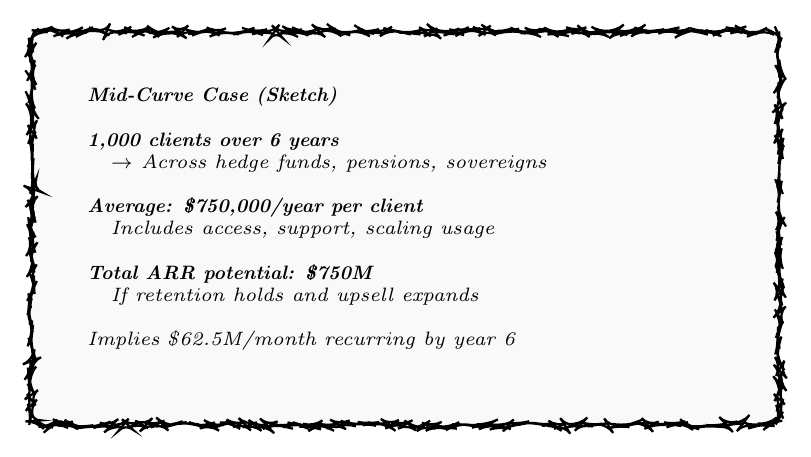
\begin{tikzpicture}[
      font=\footnotesize,
      fuzz/.style={draw=black, thick, rounded corners, fill=gray!5, decorate, decoration={random steps, segment length=2pt, amplitude=1pt}},
      txt/.style={align=left, font=\scriptsize\itshape},
    ]
  
    % Napkin box
    \node[fuzz, minimum width=9.5cm, minimum height=5cm, anchor=north west] (napkin) at (0,0) {};
  
    % Content inside
    \node[txt, anchor=north west] at ([xshift=0.6cm, yshift=-0.6cm]napkin.north west) {
      \textbf{Mid-Curve Case (Sketch)} \\
      \\
      \textbf{1{,}000 clients over 6 years} \\
      \quad $\rightarrow$ Across hedge funds, pensions, sovereigns \\
      \\
      \textbf{Average: \$750{,}000/year per client} \\
      \quad Includes access, support, scaling usage \\
      \\
      \textbf{Total ARR potential: \$750M} \\
      \quad If retention holds and upsell expands \\
      \\
      \textit{Implies \$62.5M/month recurring by year 6}
    };
  
    \end{tikzpicture}
    \caption{Napkin Sketch: Mid-curve projection for enterprise ML infrastructure revenue.}
\end{figure}

\medskip

\begin{TechnicalSidebar}{What is ARR and Why Does It Matter?}

  \textbf{ARR}, or \textit{Annual Recurring Revenue}, is a core metric for evaluating the health and scalability of 
  a subscription-based business.  
  It answers one question: \textbf{If we changed nothing, how much revenue would we make next year?}
  
  \medskip
  
  Unlike one-time sales or services, ARR assumes continuity — customers staying onboard, renewals flowing in, and 
  contracts holding steady.  
  This makes it a preferred benchmark for investors, especially in enterprise SaaS, infrastructure, and 
  fintech platforms.
  
  \medskip
  
  \textbf{Why do investors care?}

  \medskip
  
  \begin{itemize}
    \item \textbf{Predictability:} ARR provides visibility into future cash flows.
    \item \textbf{Scalability:} High ARR growth often implies network effects or strong product-market fit.
    \item \textbf{Valuation:} Many high-growth companies are valued as a multiple of ARR, not EBITDA or profit.
  \end{itemize}
  
  \medskip
  
  \textbf{Here's a back-of-envelope example:}  
  1,000 clients paying \$750K/year = \$750 million ARR.  
  If we assume a 10x revenue multiple then we get a \$7.5B potential valuation.
  
  \medskip
  
  \textit{In short: ARR is more than just a finance number.}  
  It’s the story of future certainty, told in dollars per year.
  
\end{TechnicalSidebar}

\medskip

They had moved to the bar by then. The dinner plates were cleared. Hart’s jacket was off, his sleeves pushed up, and the 
lights had dimmed just enough to signal that the crowd was thinning, but not enough to end the night.

A jazz trio murmured in the corner. Ice clinked in lowball glasses. David swirled his scotch, letting the silence stretch 
before continuing.

\medskip

``And that’s just the base stack,'' Morales said, gesturing with his glass.  
``We can spin out modules like data engines, stress frameworks, and volatility overlays.  
Each one’s a license vector. Or an acquisition target.''

Hart nodded slowly, scribbling something onto a cocktail napkin.

``At a 10x revenue multiple, that’s a \$7.5 billion ceiling.''

He looked up. ``But that’s not the point.  
The point is to scale past everyone’s comfort zone — fast enough that no one catches up.''

David leaned back, watching the amber catch in the bar light.

``You won’t get there by pitching dashboards,'' he said.  
``You need belief. You need momentum. And you need a fear of missing out.''

Hart raised his glass, smiling. ``Exactly. Blitz the market. Control the myth.''

David tapped his glass gently against Hart’s. ``You won’t get there without narrative control.''

``That’s why we’re building the narrative ourselves,'' Hart said, and drank.


\medskip

\begin{HistoricalSidebar}{The Blitzscaling Playbook: Growth First, Friction Later}

  The term \textbf{blitzscaling} was popularized by LinkedIn founder Reid Hoffman and entrepreneur Chris Yeh in their 
  2018 book of the same name.  
  It describes the strategy of prioritizing \textbf{rapid scaling over efficiency}: deliberately accepting chaos, instability, 
  and short-term loss in pursuit of long-term dominance.
  
  \medskip
  
  \textbf{The idea?} In winner-take-most markets (especially network-based or tech-driven), the biggest risk isn’t 
  inefficiency. The biggest risk is irrelevance.  

  \medskip

  The first company to reach critical scale locks in network effects, captures users, and scares off late-stage capital 
  for competitors.
  
  \medskip
  
  These are the core blitzscaling tactics:

  \medskip
  
  \begin{itemize}
    \item \textbf{Ignore traditional management advice.} Scale even when systems aren’t ready.
    \item \textbf{Outspend competitors.} Win land grabs before profit matters.
    \item \textbf{Hire ahead of revenue.} Prioritize coverage and speed over org clarity.
    \item \textbf{Fundraise fast and frequently.} Capital becomes both fuel and moat.
  \end{itemize}
  
  \medskip
  
  
  Consider the case of AirBnB. 

  \medskip
  
  In 2011–2013, AirBnB was losing money in most markets. Its customer service operations were 
  overwhelmed, and regulators were circling. However, its leadership doubled down on blitzscaling:
  
  \begin{itemize}
    \item Rapid geographic expansion to dozens of cities per quarter.
    \item Aggressive marketing with subsidized travel, and referral programs.
    \item Growing headcount, scaling trust \& safety, increasing support, and engineering all at once.
  \end{itemize}
  
  \medskip
  
  The result?

  \medskip
  
  \begin{itemize}
    \item In 2011: Airbnb was valued at \$1B.
    \item By 2014: \$10B.
    \item And by IPO in 2020: over \$100B.
  \end{itemize}
  
  \medskip
  
  Blitzscaling worked, but it wasn't without cost:  
  Legal battles, housing backlash, employee burnout, and early investor dilution were all part of the path.
  
  \medskip
  
  \textbf{The takeaway?}  
  Blitzscaling is a bet that \textit{dominance now} is worth \textit{disarray today}.  
  It’s not for every company. However, in capital-rich, timing-sensitive markets, it can be the difference between first place 
  and forgotten.
  
\end{HistoricalSidebar}


\subsection*{Editor Questions for ``The Pitch Behind the Pitch''}

To get meaningful and diverse feedback, I designed these questions to go beyond surface-level edits.
I need you to reflect not just on technical clarity or style, but on emotional resonance, character
believability, narrative structure, pacing, and thematic depth. You don’t need to answer every question.
Please focus on the ones that speak to your experience as a reader. The goal is not to fix the scene,
but to understand how it lands, where it connects, and where it might quietly miss.

\subsubsection*{Narrative \& Structure}

\begin{itemize}
\item Did the three-part arc — the pitch, the calculus, and the napkin math — feel cohesive and well-structured?
\item Did the pacing work across scenes, or did any part feel too slow or too dense?
\item Was there a clear sense of escalation or momentum across the conversations?
\item Would breaking it into more chapters or scene breaks help readability or impact?
\end{itemize}

\subsubsection*{Emotional Resonance}

\begin{itemize}
\item How did this sequence make you feel? Excited? Intrigued? Disoriented?
\item Were there moments where you felt emotionally connected to David — or distanced?
\item Did the mood and setting (e.g., scotch, jazz, marble tables) contribute meaningfully to the tone?
\end{itemize}

\subsubsection*{Character Insight}

\begin{itemize}
\item Did Hart feel like a compelling presence — someone with depth, or mostly a rhetorical device?
\item Did David feel passive or active in the negotiation? Was that satisfying?
\item How well did Morales' voice stand apart from Hart’s? Could you distinguish the characters clearly?
\end{itemize}

\subsubsection*{Thematic Cohesion}

\begin{itemize}
\item What themes did you take away from this scene? Control, access, valuation, myth?
\item Did the recurring metaphors (gateways, keycards, time arbitrage) feel earned or overused?
\item Do the technical details enhance or dilute the deeper message?
\end{itemize}

\subsubsection*{Technical \& Expository Balance}

\begin{itemize}
\item Did the technical sidebars feel integrated with the narrative or too standalone?
\item Was there any part of the explanation (e.g., synthetic credit, ARR) that dragged or confused?
\item Were the Fermi estimates and market sizing believable and satisfying as a reader?
\end{itemize}

\subsubsection*{Style \& Voice}

\begin{itemize}
\item Did the prose feel immersive, too ornate, or just right for this genre and tone?
\item Was there a line or image that stood out (positively or negatively)?
\item Did the dialogue feel stylized in a way that served the tone, or did it ever feel unnatural?
\end{itemize}

\subsubsection*{Deeper Testing}

\begin{itemize}
\item If the historical and technical sidebars were removed, how much narrative weight would be lost?
\item If this were the only chapter you read, what would you assume the book is about?
\item What kind of reader is this written for? Did you feel included, excluded, or challenged?
\end{itemize}




